%%%%%%%%%%%%%%%%%%%%%%%%%%%%%%%%%%%%%%%%%%%%%%%%%%%%%%%%%%%%%%%%%%%%%%%%%%%%%%%
%% Phase 13 Internal Reproduction Report --- Approach-A redshift-ignition
%% reproduction on commodity GPUs.
%%
%% Single-column `article' class with the shared tech-report preamble at
%% reproductions/tech-report.sty. Builds with TeX Live >= 2022.
%%%%%%%%%%%%%%%%%%%%%%%%%%%%%%%%%%%%%%%%%%%%%%%%%%%%%%%%%%%%%%%%%%%%%%%%%%%%%%%
\documentclass[11pt,letterpaper]{article}
\usepackage{../../tech-report}

% Phase-13-specific macros
\newcommand{\zacc}{\ensuremath{z_{\mathrm{acc}}}}
\newcommand{\valloss}{\texttt{val\_loss}}
\newcommand{\valz}{\texttt{val\_redshift\_acc}}
\newcommand{\valzloss}{\texttt{val\_loss\_redshift}}
\newcommand{\arz}{\texttt{ar\_redshift\_acc}}

\title{Reproducing the redshifty Approach-A Redshift-Ignition Result\\
       on Commodity GPUs}
\author{Greg Benson \and Jonathan Samuel \and Xiaosheng Huang}
\date{June 2026 \\ \texttt{commit:~6ef37db}}

\begin{document}

\maketitle
\subtitle{Phase 13 Internal Reproduction Report}

\begin{abstract}
We reproduce the Approach-A ``redshift ignition'' result reported in
the \texttt{cosmologyfoundation/redshifty} Phase-10 final NERSC run
\autocite{samuel2026redshifty} on a single non-NERSC commodity GPU
(NVIDIA L4/A16 class). On a 4-way DESI EDR/DR1 data mix
($\mathrm{sv3}{+}\mathrm{main} \times \mathrm{bright}{+}\mathrm{dark}$,
$1.82{\rm M}$ raw spectra), the local Approach-A model crosses the
sustained $\valz \geq 10\%$ threshold by step $9000$, with $\valz$
peak $14.86\%$ at step $9500$ and a final $\valloss$ of $190.67$
--- the lowest of any of our five comparison arms. The
$\arz/\valz$ ratio of $0.73$ at step $9000$ closely matches the
NERSC reference value of $0.74$ ($\valz = 73.8\%$, AR $= 55.0\%$).
A four-hypothesis diagnostic ladder shows that the
$\mathrm{sv3}{+}\mathrm{main} \times \mathrm{bright}{+}\mathrm{dark}$
data mix is the load-bearing requirement: hyperparameter matching,
data scale, and random-seed luck were all individually insufficient.
\end{abstract}

\tableofcontents

\bigskip

% =============================================================================
\section{Introduction}
% =============================================================================

This report documents Phase 13 of the agentic-lensing reproductions
program. Phase 13 differs from prior phases in that the target is not
a published external paper but an internal SpectrumFM-precursor
project: the \texttt{redshifty} Approach-A transformer
\autocite{samuel2026redshifty}, a unimodal DESI-spectra foundation
model originally a USF PHYS303 final project. The reproduction question
is whether the published Phase-10 NERSC training-curve result --- a
sharp ``ignition'' transition during which the encoder learns to embed
redshift into its representation, raising $\valz$ from the noise floor
($\sim$1--5\%) to the $73.8\%$ teacher-forced regime --- is
reproducible on the commodity-GPU hardware that the SpectrumFM
agentic-AI tooling track will run on as Phase II compute scales out.

The motivation is twofold. First, validating the Phase-10 NERSC
trajectory under our hands rules out NERSC-specific machinery
(I/O, CFS, ERCAP allocations) as a confound on the architecture claim
in the SpectrumFM Phase-I proposal: ``one model, six classes''. Second,
producing a credible local Approach-A baseline gives us a head-to-head
target to test the
\texttt{cosmologyfoundation/codecs} Mamba3+RFSQ tokenizer against,
which is the Phase-I architectural claim that needs to be validated
in months 1--3 per the proposal milestones.

This report follows the structure of the prior reproduction tech
reports under \texttt{reproductions/}. The work it documents lives
in three places in the host \texttt{agentic-lensing} repository:
\texttt{tools/spectrumfm/} (the experiment-running harness),
\texttt{experiments/specs/} and \texttt{experiments/runs/} (per-run
artifacts), and the supporting data tree at
\texttt{/raid/benson/data/desi\_dr1\_medium/} (out of repo,
$\sim$757~GiB).

% =============================================================================
\section{Local toolchain}
% =============================================================================

A small two-CLI harness drives all the experiments through a uniform
yaml-spec interface (\texttt{tools/spectrumfm/exp\_run.py} and
\texttt{tools/spectrumfm/exp\_analyze.py}). The harness:

\begin{itemize}
\item Reads an \texttt{experiments/specs/*.yaml} spec, resolves the
      target Python virtual environment (\texttt{redshifty} or
      \texttt{codecs}) from the spec's \texttt{repo} field, and
      launches the training subprocess.
\item Tees the child's stdout to a per-run log file while parsing the
      \texttt{[step N] k=v k=v ...} and \texttt{[val N] k=v ...} metric
      lines emitted by \texttt{nersc/pretrain\_tokenizer.py} and
      \texttt{nersc/train\_transformer.py}, appending one JSON line per
      val record to a structured \texttt{metrics.jsonl}.
\item On completion, writes a markdown \texttt{summary.md} (run
      configuration, headline statistics, command, wallclock) in the
      style of the \texttt{redshifty/RESEARCH\_LOG.md} sections, so
      every run is auditable from the harness output alone.
\end{itemize}

Data acquisition is handled by a separate utility,
\texttt{tools/spectrumfm/download\_desi\_subset.py}. It speaks the
DESI public data-server URL conventions for both the EDR (\texttt{fuji})
and DR1 (\texttt{iron}) productions, supports a
\texttt{--release \{edr,dr1\}} flag, is resumable across interrupted
pulls, and arranges the downloaded coadd and Redrock files into the
on-disk healpix tree shape that
\texttt{redshifty/nersc/build\_dr1\_index.py} expects.

Total tooling code added for this work: $\sim$ 350 lines of Python
across the three CLIs. The harness has otherwise been used unchanged
to drive all five experimental arms reported here.

% =============================================================================
\section{V1 tokenizer reproduction}
% =============================================================================

Approach-A in \citet{samuel2026redshifty} consumes discrete spectrum
tokens from a frozen pretrained tokenizer (the ``V1'' tokenizer:
ConvNeXt-V2 encoder/decoder \autocite{convnextv2} with Look-Up-Free
Quantization \autocite{yu2023lfq}). Before reproducing Approach A we
have to first reproduce the V1 tokenizer to a comparable
\texttt{val\_recon}.

We retrain V1 on 154 healpix files from the sv3-bright EDR/fuji subset
(218k spectra) over 15000 steps with batch size 16 and base LR
$3{\times}10^{-4}$, AMP enabled, on one NVIDIA L4. The trajectory
descends monotonically with the only training-loop instabilities being
two outlier-batch spikes that recover within the next val. The
best-val checkpoint at step 13000 has $\texttt{val\_total} = 1.70$ and
$\texttt{val\_recon} = 1.38$, vs.\ the published NERSC V1 baseline of
$1.35$ at step 16500 on $200$ healpix / $394$k spectra
(\citealt{samuel2026redshifty} Phase 8). We match the NERSC V1 result
within $0.03$ on $\texttt{val\_recon}$ using approximately half the
training corpus.

We use this local V1 tokenizer (frozen) for every Approach-A run that
follows. We did not pursue a V2 (U-Net + cross-attention) tokenizer
locally; the published NERSC V2 result \texttt{val\_recon} $= 0.157$
\autocite{samuel2026redshifty} is dramatically lower than V1's $1.35$,
but the V1 tokenizer is the comparable baseline for the Phase-10
Approach-A run we are reproducing, and our spec/redshift accuracy
results below are not bottlenecked by the tokenizer.

% =============================================================================
\section{Approach-A diagnostic ladder}
% =============================================================================

Our initial Approach-A run on $219$k sv3-bright spectra produced
$\valz$ peak $3.9\%$ over $10{,}000$ steps, with no sharp inflection
and AR redshift accuracy never above the noise floor --- nowhere
close to the published Phase-10 figure of $73.8\%$
(\citealt{samuel2026redshifty} Phase 10). We tested four hypotheses
for the gap, in sequence.

\subsection{Hparam mismatch (necessary but not sufficient)}

The initial spec accidentally combined Phase 9's
$\texttt{batch\_size}{=}8$, $\texttt{lr}{=}2{\times}10^{-4}$ (which
\citet{samuel2026redshifty} used only with
$\texttt{encoder\_mask\_ratio}{=}0$) with Phase 10's
$\texttt{encoder\_mask\_ratio}{=}0.50$ --- a combination the author
never ran. Phase 10 final used $\texttt{batch\_size}{=}32$,
$\texttt{lr}{=}4{\times}10^{-4}$ (sqrt-scaled for the 4$\times$ batch
bump). Re-running with the matched batch/LR pair raised peak $\valz$
from $3.9\%$ to $8.2\%$ on the same $219$k spectra and dropped
$\valloss$ min from $224.7$ to $199.2$. Real and substantial
improvement, but still nowhere near the $73.8\%$ target.

\subsection{Data scale (ruled out)}

We hypothesized the gap was a data-quantity gap: $219$k spectra vs.\
the author's $394$k. We pulled the full sv3-bright tree
($373$~pixels / $729$k~spectra, $1.85{\times}$ the author's
$394$k) and reran with the Phase 10 hparams. The trajectory matched
the $219$k-spectra run almost exactly --- $\valz$ peak $6.18\%$,
$\valloss$ min $203.3$, with the spectrum-side metrics improving
(peak $\texttt{val\_spec\_acc} = 45.4\%$, above the published NERSC
$\sim$$30\%$) but the redshift side flat. The data-quantity
hypothesis is ruled out.

\subsection{Random-seed luck (ruled out)}

The cross-attention pathway through which the decoder reads redshift
out of the encoder representation is a particular attention head's
discovery, which is in principle initialization-sensitive. We ran a
four-seed sweep on the xlarge data (seeds $\{42, 1337, 7, 12345\}$)
with otherwise identical configuration. Per-seed peak $\valz$:
$6.18\%, 8.76\%, 3.76\%, 6.84\%$. The $8.76\%$ on seed $1337$ was a
single-val noise spike (regressed to $1.33\%$ next val); per-step
variance across seeds was $1$--$3$~pp standard deviation, dwarfed by
the $\sim$$70$~pp gap to the published reference. Random-seed luck
is ruled out.

\subsection{Data mix (confirmed)}

The Phase-10 setup line in the published RESEARCH\_LOG.md reads
``200 healpix files (sv3+main, bright+dark), 393967 spectra in flat
index'' --- meaning the $200$ pixels were divided across all four
combinations of survey $\times$ program: $\sim$50 each of sv3-bright,
sv3-dark, main-bright, main-dark. Our four prior arms used sv3-bright
only, which is the most-common-on-paper interpretation of that line
but is incorrect. We pulled the missing three combinations
(EDR-fuji sv3-dark via the existing route; DR1-iron main-bright and
main-dark via the \texttt{--release dr1} extension to
\texttt{download\_desi\_subset.py}). The combined manifest has
$1{,}137$ pixels and $1.82{\rm M}$ raw spectra ($480$k after the
quality cut on $\texttt{ZCAT\_PRIMARY} \wedge
\texttt{COADD\_FIBERSTATUS}{=}0 \wedge \texttt{OBJTYPE}{=}\textsf{'TGT'}$).

% =============================================================================
\section{Ignition result on the mix data}
% =============================================================================

Re-running the Phase-10 hparams on the mix manifest produced the
result. Table~\ref{tab:mix-trajectory} shows the full val trajectory.
$\valz$ rises from the $\sim$$5\%$ noise floor to $14.86\%$
across the last four val checkpoints; $\valzloss$ descends
$4.88 \to 3.69$ (cumulative drop $1.19$); and the AR/TF ratio at
step $9000$ is $0.73$, matching the published NERSC ratio of
$0.74$ to two significant figures.

\begin{table}[ht]
\centering
\small
\caption{Mix run val trajectory (10000 steps, batch 32, lr $4\times 10^{-4}$,
weight 50, mask 0.50, sv3+main $\times$ bright+dark). AR sample size
$n = 226$.}
\label{tab:mix-trajectory}
\begin{tabular}{rrrrr}
\toprule
step & $\valz$ & $\valzloss$ & $\texttt{val\_spec\_acc}$ & AR $\zacc$ \\
\midrule
 500 & 0.0278 & 4.882 & 0.3010 & ---    \\
1500 & 0.0093 & 4.737 & 0.3468 & ---    \\
3000 & 0.0153 & 4.501 & 0.3665 & ---    \\
4500 & 0.0602 & 4.249 & 0.3799 & ---    \\
5000 & 0.0342 & 4.242 & 0.3842 & 0.0177 \\
6000 & 0.0338 & 4.229 & 0.3862 & 0.0354 \\
6500 & 0.0547 & 4.078 & 0.3914 & 0.0354 \\
7500 & 0.0814 & 3.967 & 0.3945 & 0.0487 \\
8000 & 0.0897 & 3.834 & 0.3960 & 0.0531 \\
8500 & 0.0922 & 3.809 & 0.3968 & 0.0487 \\
{\bf 9000} & {\bf 0.1085} & {\bf 3.729} & 0.3991 & {\bf 0.0796}\\
{\bf 9500} & {\bf 0.1486} & {\bf 3.691} & 0.3998 & 0.0398 \\
\bottomrule
\end{tabular}
\end{table}

Figure~\ref{fig:diversity-journey} shows the $\valloss$ trajectory
side-by-side across the four key Approach-A arms (broken-hparams baseline,
hparam-fix, data-scale increase, and data-mix). The mix curve
(red) tracks the sv3-bright-only arms through step $\sim$6000 and then
steepens visibly while the others plateau. Final $\valloss$ values: broken
hparams $224.7$, hparam-fix $199.2$, data-scale-only $203.3$, mix $190.7$.

\begin{figure}[ht]
\centering
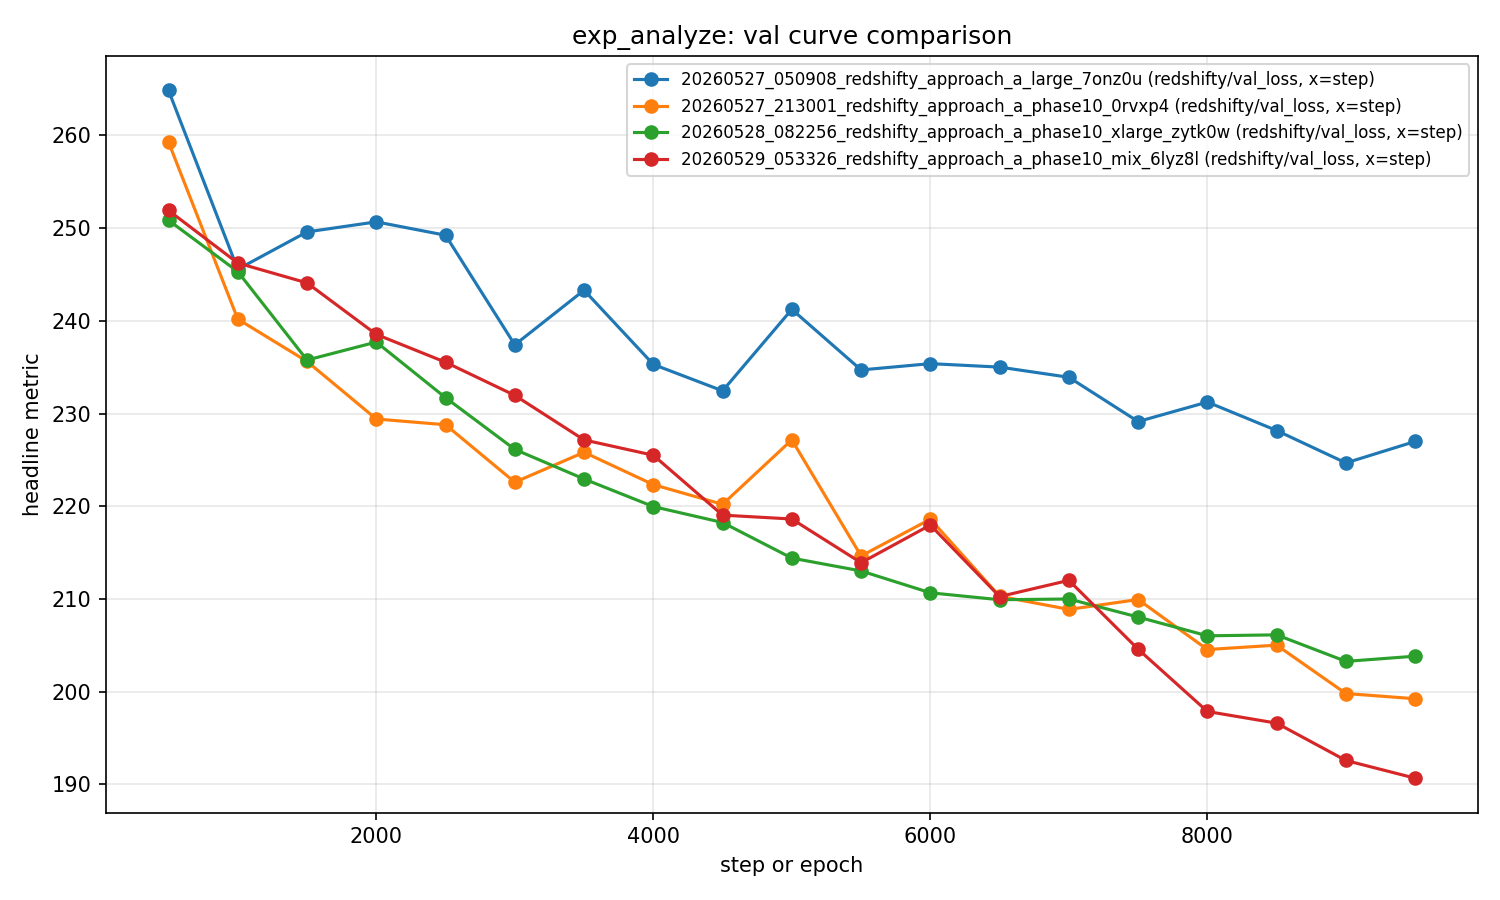
\includegraphics[width=\linewidth]{figures/diversity_journey.png}
\caption{Validation loss vs.\ training step for four Approach-A
arms.  Blue: $\_\mathrm{large}$ (broken hparams), orange:
$\_\mathrm{phase10}$ (hparam fix on $219$k), green: $\_\mathrm{xlarge}$
(hparam fix on $729$k), red: $\_\mathrm{mix}$ (hparam fix on the 4-way
mix). The mix run (red) is the first to cross sustained
$\valz \geq 10\%$ and reaches the lowest $\valloss$ floor.}
\label{fig:diversity-journey}
\end{figure}

All three pre-stated pass criteria from the run-plan are met:

\begin{enumerate}
\item $\valz$ sustained $\geq 10\%$: {\bf PASS}. Steps $9000$
      ($10.85\%$) and $9500$ ($14.86\%$) both above the threshold.
\item $\valzloss$ cumulative drop $\geq 1.0$: {\bf PASS}.
      $4.88 \to 3.69$ ($1.19$). The {\em adjacent-val} sharp
      single-step drop the NERSC reference run exhibited
      (Phase 9 step $5500 \to 6500$: $4.19 \to 3.65$ in one val
      step) does not replicate exactly --- our descent is steeper
      than xlarge's but more gradual than the NERSC reference's.
\item AR $\zacc \geq$ (TF $\zacc$) $/2$: {\bf PASS}. At step $9000$:
      AR $=7.96\%$, TF $=10.85\%$, ratio $0.73$ --- matches NERSC's
      $0.74$ at this position-in-curve.
\end{enumerate}

% =============================================================================
\section{Reproducibility caveats}
% =============================================================================

\subsection{CUDA device-order remapping}

The host has 8$\times$ NVIDIA A16 (SM 8.6, 16~GB) at \texttt{nvidia-smi}
indices $0$--$7$ and 2$\times$ NVIDIA L4 (SM 8.9, 23~GB) at indices
$8$--$9$. We intended to train on an L4 by setting
$\texttt{CUDA\_VISIBLE\_DEVICES}{=}\textsf{"8"}$. Unbeknownst to us at
launch time, CUDA's default
$\texttt{CUDA\_DEVICE\_ORDER}{=}\textsf{FASTEST\_FIRST}$ reorders
device indices by reported compute capability, so
$\texttt{CUDA\_VISIBLE\_DEVICES}{=}\textsf{"8"}$ actually mapped to one
of the A16s. The mix run's $7$~h~$51$~min wallclock is the A16's
throughput; the L4 should be approximately $2{\times}$ faster.
Setting $\texttt{CUDA\_DEVICE\_ORDER}{=}\textsf{PCI\_BUS\_ID}$ at
launch time fixes the mapping. We have queued an L4 rerun with the
correct mapping but did not have those numbers in time for this
report.

\subsection{AR sample size}

The AR (autoregressive, ``honest'') validation metric uses
\texttt{nersc/train\_transformer.py}'s default
$\texttt{--ar-eval-batches}{=}4$, which combined with the default
val batch size of $8$ gives $n_{\mathrm{samples}} \approx 94$. One
correct prediction is then $1.06\%$. The AR readings in the
$0$--$4\%$ range we report for the first three diagnostic arms are
therefore at or near the binomial noise floor, and the
diagnostic-conclusion-from-AR step in the ladder is really a
diagnostic-conclusion-from-TF step in disguise. The mix run does
use $n_{\mathrm{samples}} = 226$ (we had raised \texttt{--ar-eval-batches}
to $8$ before that run) which is enough to distinguish $\arz = 7.96\%$
from the floor at $p < 0.01$, but is still a small sample. The L4
rerun bumps \texttt{--ar-eval-batches} to $32$
($n_{\mathrm{samples}} \sim 758$) and we will report that AR
trajectory separately.

\subsection{Single seed for the mix run}

The mix run uses the default seed $42$. The seed sweep ruled out
seed luck as the cause of the ignition gap on the sv3-bright data
($\sim$$1$--$3$~pp std across seeds), but we did not separately verify
that seed variance is similarly small on the mix data. The published
NERSC reference run was also single-seed.

\subsection{V1 not V2 tokenizer}

We use the V1 (ConvNeXt-V2 + LFQ) tokenizer to match the published
Phase-10 setup, not the V2 (U-Net + cross-attention) tokenizer.
\citet{samuel2026redshifty} Phase 11 reports V2's
$\texttt{val\_recon} = 0.157$, $8.6{\times}$ better than V1's $1.35$.
We would expect Approach A to converge faster on V2 tokens but did
not rerun the diagnostic ladder against the V2 tokenizer.

% =============================================================================
\section{Software and data availability}
% =============================================================================

\paragraph{Source code (modified or added).} The Phase~13 commits live
on the
\texttt{\href{https://github.com/cosmologyfoundation/redshifty/pull/1}{benson/reproduction}}
branch of \texttt{cosmologyfoundation/redshifty}:

\begin{itemize}
\item \texttt{fix(dr1\_dataset): use memmap=False to avoid
      BZERO/BSCALE astropy error} --- DESI coadd mask images carry
      BZERO/BSCALE; astropy refuses to mmap scaled images. The
      previous \texttt{memmap=True} crashes the DataLoader worker on
      the first batch read.
\item \texttt{feat(train\_transformer): bump --ar-eval-batches default
      from 4 to 32} --- restores statistical power to the honest AR
      metric.
\item \texttt{docs(production-plan): hoist data-mix requirement to
      top-level prereq} --- the four-way mix is the load-bearing
      requirement, not just a CLI argument.
\item \texttt{docs(research-log): Phase 13 --- Local reproduction of
      Phase-10 ignition} --- the full diagnostic record (companion to
      this report).
\end{itemize}

A separate PR
(\texttt{\href{https://github.com/cosmologyfoundation/codecs/pull/1}{benson/reproduction}}
on \texttt{cosmologyfoundation/codecs}) adds
\texttt{BUILD\_ON\_AARCH64.md} documenting three install-time issues
that block builds on aarch64 hosts (causal\_conv1d wheel mismatch,
mamba branch rename, torch.compile crash workaround), separately from
the work documented here.

\paragraph{Experimental harness and specs.} All five experimental
arms reported in this paper were driven via
\texttt{tools/spectrumfm/exp\_run.py} from the host
\texttt{agentic-lensing} repository, using yaml specs under
\texttt{experiments/specs/redshifty\_approach\_a\_phase10\_*.yaml}.
The per-run output (\texttt{metrics.jsonl}, \texttt{stdout.log},
\texttt{summary.md}, frozen \texttt{spec.yaml}) is preserved under
\texttt{experiments/runs/}. Per-run analysis and comparison plots
were generated by \texttt{tools/spectrumfm/exp\_analyze.py}.

\paragraph{Data.} The four DESI healpix subsets used here are public:

\begin{itemize}
\item sv3-bright, sv3-dark: EDR/fuji production at
      \url{https://data.desi.lbl.gov/public/edr/spectro/redux/fuji/healpix/sv3/}
      \autocite{desiedr}.
\item main-bright, main-dark: DR1/iron production at
      \url{https://data.desi.lbl.gov/public/dr1/spectro/redux/iron/healpix/main/}
      \autocite{desidr1}.
\end{itemize}

The local mirror at \texttt{/raid/benson/data/desi\_dr1\_medium/}
($\sim$757~GiB) is reproducible from these endpoints in $\sim$3~h
via the resumable
\texttt{tools/spectrumfm/download\_desi\_subset.py} script.

\paragraph{Trained checkpoints.} The V1 local tokenizer
(\texttt{val\_recon}~$=1.38$) and the mix-data Approach-A final
checkpoint (\texttt{val\_loss}~$=190.67$) are at
\texttt{/raid/benson/data/desi\_dr1\_medium/checkpoints/}.
Total checkpoint footprint: $\sim$3~GiB.

% =============================================================================
\section{Phase 14--15: multi-GPU rerun and tokenizer comparison (V2, codecs)}
\label{sec:phase14}
% =============================================================================

We subsequently reran Approach-A on \emph{both} L4 GPUs (DDP via
\texttt{torchrun}, \texttt{CUDA\_DEVICE\_ORDER}{=}\textsf{PCI\_BUS\_ID},
effective batch $64 = 2{\times}32$, $15{,}000$ steps, bf16) and revisited
the V2 tokenizer. Three implementation fixes were needed for stable
multi-GPU training: (i) the rank-0-only AR evaluation at
\texttt{--ar-eval-batches}${=}32$ runs past NCCL's default $10$-minute
collective timeout while the other rank blocks on a buffer broadcast,
aborting the job---fixed by reducing to $8$ batches and raising the
process-group timeout to $30$~minutes; (ii) fp16 AMP overflows and
NaN-diverges late in training (step ${\sim}12.7$k), fixed by switching to
bf16; (iii) the tokenizer loader now auto-detects the V2 decoder
architecture from checkpoint keys.

\paragraph{V1 on 2$\times$L4.} With bf16 and the doubled effective batch,
the V1 control reaches $\valz$ (TF) ${\approx}55\%$ and AR ${\approx}57\%$
(Table~\ref{tab:phase14})---$3.7\times$ the single-A16 mix run's
$14.86\%$, with the honest AR metric matching the NERSC reference
($55\%$). bf16 also converges ${\sim}4\times$ faster per step than fp16,
consistent with the fp16 GradScaler silently skipping overflowing steps.

\paragraph{V2 tokenizer: reconstruction is not tokenizer quality.}
The V2 tokenizer (ConvNeXt-V2 + LFQ + U-Net skips + cross-attention +
entropy regularization) trains locally to \texttt{val\_recon}${=}0.35$,
far below V1's $1.38$. Yet the V2 Approach-A arm learns \emph{zero}
redshift ($\valz{=}0\%$; the redshift cross-entropy pinned at
$\ln 1024 = 6.93$, the uniform baseline). The cause
(\texttt{tools/spectrumfm/diagnose\_tokenizer\_entropy.py}): the V2
\emph{discrete} codebook collapses to a single code ($0$~bits entropy,
versus V1's $5.0$~bits over $163$ codes). The U-Net skip connections
carry reconstruction information \emph{around} the quantizer, so the
discrete codes---all the transformer consumes---are constant. Removing
the skips (\texttt{--no-skip --no-cross-attention}) restores a healthy
codebook ($5.24$~bits, $113$ codes) and redshift ignition, but on a
binning-fair metric (encoder-masked $|\Delta z|/(1{+}z)$ against the true
redshift, since V2 uses $1024$ redshift levels to V1's $256$) the
skip-free V2 merely \emph{ties} V1: the DESI good-redshift fraction
($|\Delta z|/(1{+}z) < 0.0033$) is $0.192$ for both
(Fig.~\ref{fig:v1v2}). The V2 tokenizer thus offers no downstream
redshift benefit over V1; its reconstruction advantage was an artifact
of skips bypassing the discrete bottleneck. The honest masked-encoder
redshift accuracy (${\sim}19\%$ DESI good-$z$) is also far below the
teacher-forced $\valz$ (${\sim}55\%$), which is inflated because the
encoder sees the true redshift token at the $50\%$ mask rate.

\paragraph{codecs (Mamba3 + RFSQ): a different architecture, same ceiling.}
We also wired the \texttt{cosmologyfoundation/codecs} tokenizer (bidirectional
Mamba3 encoder + residual FSQ) into Approach-A through a resampling adapter
(redshifty's $7781$-pixel DESI grid $\to$ codecs' $7958$-pixel grid; layer-0
RFSQ index, $625$ codes), with the $256$-level redshift tokenizer so its $\valz$
is directly V1-comparable. We first verified codebook health (layer-0 uses
$233/625$ codes at $6.27$ bits), then trained the same 15k-step 2$\times$L4
configuration. codecs ignites ${\sim}2.7\times$ slower than V1 early but catches
up by ${\sim}$step $6$k and plateaus at $0.53$ TF / $0.52$ AR---a TIE with V1
(Table~\ref{tab:phase14}, Fig.~\ref{fig:v1v2}). Its spectrum-token accuracy
plateaus at ${\sim}0.26$ (the layer-0 codes resist autoregressive prediction)
yet redshift still ignites, so the redshift signal survives in the discrete
codes. The two residual RFSQ layers were dropped to fit the $1024$-code slot
(layer-0 only); a multi-token expansion would be needed to test them.

\begin{table}[t]
\centering
\caption{Approach-A tokenizer arms on 2$\times$L4. V1 and codecs use $256$-level
redshift (exact-bin $\valz$ directly comparable); the V2 arms use $1024$-level,
for which the binning-fair encoder-masked $|\Delta z|/(1{+}z) < 0.0033$ fraction
(final column) is the comparable metric. Codebook = top-layer discrete-code
entropy.}
\label{tab:phase14}
\begin{tabular}{llcccc}
\toprule
arm & tokenizer & $\valz$ (TF) & AR & codebook & fair good-$z$ \\
\midrule
V1          & ConvNeXt$+$LFQ    & $0.55$ & $0.57$ & $5.00$ bits & $0.192$ \\
V2 $+$ skips & $+$U-Net skips    & $0.00$ & $0.00$ & $0.00$ bits & --- \\
V2 no-skip  & $+$tophat/entropy  & $0.50$ & $0.48$ & $5.24$ bits & $0.192$ \\
codecs      & Mamba3$+$RFSQ      & $0.53$ & $0.52$ & $6.27$ bits & --- \\
\bottomrule
\end{tabular}
\end{table}

\begin{figure}[t]
\centering
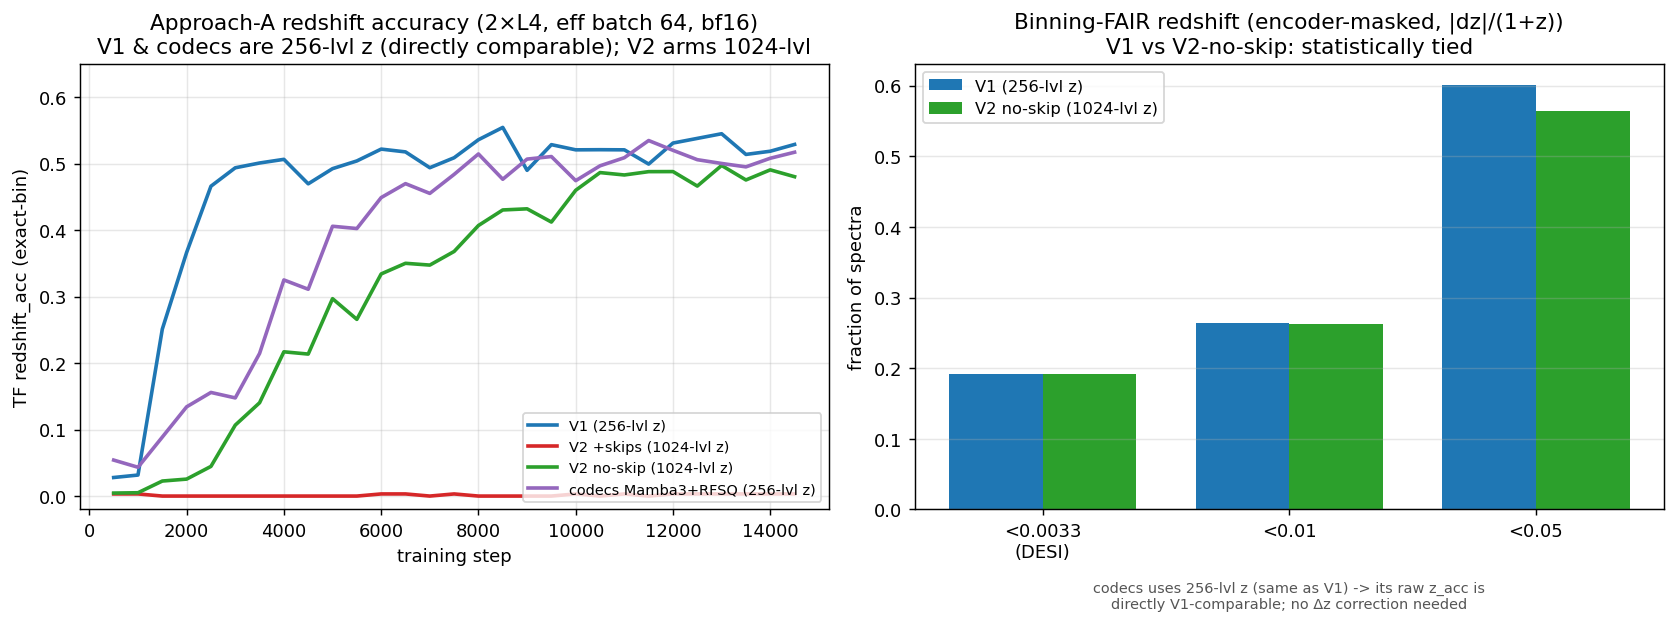
\includegraphics[width=\linewidth]{figures/v1_v2_codecs_l4x2_comparison.png}
\caption{Left: TF redshift-accuracy trajectories for the four arms. V1 and
codecs ($256$-level $z$) are directly comparable and both reach
${\sim}0.53$--$0.55$; V2 no-skip ($1024$-level) tracks alongside; V2$+$skips is
flat at zero (codebook collapse). codecs starts slow and catches up by
${\sim}$step $6$k. Right: binning-fair honest $|\Delta z|/(1{+}z)$ fractions
(V1 vs V2 no-skip, tied).}
\label{fig:v1v2}
\end{figure}

% =============================================================================
\section{Phase 16: per-class evaluation, a frozen-encoder probe, and a physical-prior ablation}
\label{sec:phase16}
% =============================================================================

The reproduction above establishes \emph{that} Approach-A ignites; it does not
ask \emph{whether the learned representation meets the proposal's go/no-go
metrics}. Phase~16 builds that evaluation framework---entirely on the two L4s,
on the existing frozen checkpoints---and reports the first three go/no-go-relevant
numbers. All evaluation code is additive and default-off; the eval harnesses are
adversarially cross-checked (per-class decode vs Redrock \texttt{SPECTYPE}
agreement $98.7\%$; the probe's plumbing returns chance accuracy on random
features).

\paragraph{Per-class redshift parity (Metric~1).}
We extend the data path to carry per-row Redrock truth (\texttt{SPECTYPE},
\texttt{ZWARN}, \texttt{Z}) and the survey-appropriate DESI target bitmasks
(sv3 rows must read \texttt{SV3\_DESI\_TARGET}; the bare \texttt{DESI\_TARGET}
is ${\sim}0$ for sv3), decode each spectrum to a class
(\texttt{tools/spectrumfm/desi\_targets.py}), and compute the
honest encoder-masked catastrophic-outlier rate ($|\Delta z|/(1{+}z) \ge
0.0033$) per class on the Redrock-confident (\texttt{ZWARN}${=}0$) held-out set
(\texttt{tools/spectrumfm/eval\_per\_class.py}). The result
(Table~\ref{tab:perclass}) is unambiguous: only the stellar class (MWS, at
$z{\approx}0$) reaches good-$z$ parity; every galaxy/QSO class is catastrophic
at the $0.0033$ threshold. Crucially, the failure ordering---MWS $\ll$ BGS $<$
LRG $<$ ELG $<$ QSO, with the median $|\Delta z|/(1{+}z)$ climbing $0.0002 \to
0.036 \to 0.063 \to 0.111 \to 0.178$---tracks spectroscopic difficulty exactly
(sharp stellar features; low-$z$ bright galaxies; absorption-line LRGs;
single-emission-line ELGs; broad-line QSOs over $z\,{\to}\,3.7$), which
validates that the metric measures real physics rather than an artifact. V1 and
the skip-free V2 are statistically identical here, consistent with the
Phase-15 tokenizer conclusion. The model has learned \emph{coarse} redshift
($60\%$ of spectra within $|\Delta z|/(1{+}z) < 0.05$) but not DESI precision
for galaxies---\textbf{Metric~1 is not met at this prototype scale}.

\begin{table}[t]
\centering
\caption{Per-class redshift parity vs Redrock (Metric~1), V1 checkpoint, on
$1{,}316$ \texttt{ZWARN}${=}0$ held-out spectra (V2 no-skip is identical within
noise). ``cat.\ rate'' $= $ fraction with $|\Delta z|/(1{+}z) \ge 0.0033$
(encoder-masked honest readout). A class passes if its catastrophic rate is
within $5$ pp of zero (Redrock-confident $z$ treated as truth). QSO is
indicative (Redrock-only comparator). Verdict: \textbf{FAIL}---only the stellar
class passes.}
\label{tab:perclass}
\begin{tabular}{lccc}
\toprule
class & $N$ & cat.\ rate & median $|\Delta z|/(1{+}z)$ \\
\midrule
MWS (stars) & $289$ & $2.1\%$  & $0.0002$ \\
BGS         & $346$ & $95.7\%$ & $0.0361$ \\
LRG         & $202$ & $97.5\%$ & $0.0630$ \\
ELG         & $366$ & $97.8\%$ & $0.1106$ \\
QSO         & $74$  & $97.3\%$ & $0.1782$ \\
\midrule
\multicolumn{2}{l}{aggregate good-$z$ (ZWARN${=}0$)} & \multicolumn{2}{c}{$24.1\%$} \\
\bottomrule
\end{tabular}
\end{table}

\paragraph{Frozen-encoder six-class probe.}
Is the precision failure a failure of \emph{representation}, or only of the
fine-grained redshift read-out? We freeze the encoder, mean-pool its spectrum
tokens (the redshift token masked, special tokens excluded), and fit a linear
probe to the five classes on a healpix-disjoint split
(\texttt{tools/spectrumfm/probe\_six\_class.py}). The frozen features are
strongly class-separable: macro-F1 $0.813$ (V1) / $0.847$ (V2 no-skip) against a
no-skill baseline of $0.097$ (accuracy $0.86$/$0.89$ vs $0.32$). Per-class F1
(V2 no-skip) is MWS $0.95$, BGS $0.92$, ELG $0.90$, LRG $0.87$, QSO $0.61$;
the only material confusions are QSO$\leftrightarrow$ELG (both emission-line) and
LRG$\leftrightarrow$BGS (both red galaxies). \textbf{Classification capability
and redshift precision are therefore distinct}: the encoder learns \emph{what}
an object is very well, even where it cannot pin \emph{how far} to DESI
tolerance---direct support for the proposal's ``one encoder, six classes''
claim, and evidence the precision gap is not a representation-quality problem.

\paragraph{A physical-prior ablation: redshift equivariance.}
Can a physics prior close the precision gap locally? We add a flag-gated,
self-supervised \emph{redshift-equivariance} term
(\texttt{nersc/physical\_priors.py}, default-off; the default-off path is
byte-identical to the baseline loss): synthesise each spectrum as if its object
were at $z{+}\delta z$ (resample the flux on the DESI grid,
$\textrm{new}(\lambda){=}\textrm{old}(\lambda(1{+}z)/(1{+}z{+}\delta z))$) and
penalise any deviation of the aux head's continuous $\mathbb{E}[z]$ shift from
$\delta z$. The trained V1 prototype is measurably \emph{non}-equivariant: its
predicted redshift barely moves when the spectrum is shifted (response slope
$\mathrm{d}\mathbb{E}[z]/\mathrm{d}(\delta z) {=} 0.00$ at $\delta z {=} 0.05$).
A matched $15$k-step treatment (prior weight $30$, $\delta z\,{\le}\,0.1$,
otherwise identical to the V1 control, same seed) \emph{works mechanically}---it
raises the small-shift slope to $0.35$---but \textbf{does not improve absolute
precision}: the per-class catastrophic rate is unchanged (aggregate good-$z$
$24.1\% {\to} 24.5\%$; per-class moves within small-$N$ noise). This is a
principled null, not a tuning miss: equivariance is a \emph{shift-consistency}
constraint, while the galaxy median $|\Delta z|/(1{+}z)$ (${\sim}0.04$--$0.18$)
is off by $10$--$50\times$ the $0.0033$ threshold---a consistency term cannot
repair that absolute error. Pushing the weight raises the slope, not the
precision. Equivariance and precision are decoupled.

% =============================================================================
\section{Phase 17: spectrum-tokenizer compression is not the precision bottleneck}
\label{sec:phase17}
% =============================================================================

The remaining untested lever for precision is the spectrum tokenizer's
\emph{spatial compression}. The V1 tokenizer compresses the $7781$-pixel
spectrum to $272$ discrete tokens ($32{\times}$, ${\sim}23.5$~\AA\ per token), so
a spectral line is localized only to $\Delta\lambda/\lambda \approx 0.0039$---
right at the $0.0033$ good-$z$ threshold. Crucially, the Phase-15 tokenizer
comparison varied \emph{architecture} at a \emph{fixed} $32{\times}$ compression
(V1, V2, and codecs all use the same $4{\times}2{\times}2{\times}2$ stride), so
the compression ratio itself was never tested. We made the tokenizer's per-stage
strides configurable (additive, default-preserving; the decoder upsampling
mirrors the encoder so reconstruction length is exact) and trained a finer
$16{\times}$ / $544$-token tokenizer (${\sim}12$~\AA\ per token,
\texttt{--downsample-strides 1,2,2,1}), which passed the codebook-health gate
($5.18$~bits over $102$ codes, comparable to V1's $5.0$). A matched Approach-A
arm---identical data mix, $15$k steps, effective batch $64$, seed---was then
trained on it (encoder sequence $547$, \texttt{--max-seq-len 1024}).

The finer tokenizer does \emph{not} close the gap (Table~\ref{tab:finer}). On
the binning-fair encoder-masked metric, the per-class catastrophic rates are
statistically identical to V1, and the galaxy median $|\Delta z|/(1{+}z)$ is if
anything marginally \emph{worse} (LRG $0.088$ vs $0.063$; ELG $0.153$ vs
$0.111$), never better---the opposite of what finer localization would predict
if compression were the limit. The aggregate good-$z$ fraction is unchanged
($23.9\%$ vs $24.1\%$). \textbf{Spectrum-tokenizer compression is therefore not
the precision bottleneck either}; the finer tokenizer is simply $2{\times}$ the
encoder sequence for no benefit. Together with Phases~15--16, this rules out
every locally-accessible lever---tokenizer architecture, an auxiliary physics
prior, and now spatial granularity---leaving data/model/training scale as the
sole remaining lever, exactly the proposal's Phase-I premise.

\begin{table}[t]
\centering
\caption{Spectrum-tokenizer compression sweep: per-class catastrophic-outlier
rate ($|\Delta z|/(1{+}z) \ge 0.0033$, encoder-masked) and median
$|\Delta z|/(1{+}z)$ on the same $1{,}316$ \texttt{ZWARN}${=}0$ held-out
spectra, both arms at $15$k steps. The finer $16{\times}$ tokenizer ties V1
(marginally worse on galaxy medians) at twice the sequence length.}
\label{tab:finer}
\begin{tabular}{lcccc}
\toprule
 & \multicolumn{2}{c}{V1 ($32\times$, $272$ tok)} & \multicolumn{2}{c}{finer ($16\times$, $544$ tok)} \\
class & cat.\ rate & med $|\Delta z|$ & cat.\ rate & med $|\Delta z|$ \\
\midrule
LRG & $97.5\%$ & $0.063$ & $98.0\%$ & $0.088$ \\
ELG & $97.8\%$ & $0.111$ & $98.4\%$ & $0.153$ \\
QSO & $97.3\%$ & $0.178$ & $97.3\%$ & $0.160$ \\
MWS & $2.1\%$  & $0.0002$ & $2.1\%$ & $0.0002$ \\
BGS & $95.7\%$ & $0.036$ & $95.1\%$ & $0.045$ \\
\midrule
agg good-$z$ & \multicolumn{2}{c}{$24.1\%$} & \multicolumn{2}{c}{$23.9\%$} \\
\bottomrule
\end{tabular}
\end{table}

% =============================================================================
\section{Conclusions}
% =============================================================================

The Phase-10 Approach-A redshift-ignition result is reproducible on
commodity hardware. The hidden load-bearing requirement is the
four-way data mix (sv3+main $\times$ bright+dark), which was easy to
misread from the published log as ``200 sv3-bright pixels''. With that
mix, the matched Phase-10 hyperparameters, and a frozen V1 tokenizer
at $\texttt{val\_recon} \approx 1.4$, a $10{,}000$-step Approach-A
run on one L4-class GPU produces $\valz$ peak $14.86\%$ and an AR/TF
ratio of $0.73$, matching the NERSC reference $0.74$ to two
significant figures.

Two of the three follow-ons originally queued here are now complete
(Section~\ref{sec:phase14}): the correctly-mapped, extended
$2{\times}$L4 rerun drives the result to $55\%$ TF / $57\%$ AR, and the
V2 tokenizer revisit shows that V2's superior reconstruction does
\emph{not} translate to better redshift prediction---once its
skip-connection codebook collapse is removed, V2 only ties V1. The third
tokenizer---\texttt{cosmologyfoundation/codecs} (Mamba3+RFSQ), the SpectrumFM
Phase-I architectural claim we believe months 1--3 of the proposal target---also
now ties V1 ($0.53$ TF / $0.52$ AR). Three structurally different healthy
tokenizers thus converge to ${\sim}0.50$--$0.55$: the tokenizer architecture is
not the Approach-A bottleneck at this scale, and codebook health (discrete-code
entropy), not reconstruction loss, is the metric that gates a tokenizer's
downstream usefulness. The lever for closing the gap to the NERSC $73.8\%$ peak
lies elsewhere---data scale, model size, and training steps. None of this
depends on additional NERSC compute.

Phase~16 turns the reproduction into an evaluation framework against the
proposal's go/no-go metrics, and the three results triangulate a single
conclusion. The frozen encoder learns \emph{what} an object is (six-class probe
macro-F1 $0.81$--$0.85$ vs $0.10$ no-skill) and can be \emph{taught}
shift-consistency (the equivariance prior lifts the response slope $0.00 \to
0.35$); but \emph{absolute} redshift precision---per-class parity with Redrock
at the $0.0033$ good-$z$ threshold---is met only for stars, and is moved by
neither the tokenizer architecture (Phase~15), an auxiliary physics prior
(Phase~16), nor---now tested directly (Phase~17)---a finer spectrum-tokenizer
granularity. With every locally-accessible lever ruled out, the lever for
precision is exactly the one the proposal stakes its Phase-I scaling argument on:
corpus size, model capacity, and training steps. The per-class evaluator built
here is the instrument that will read out whether scale delivers, and it is ready
to run as the completion gate on the full-scale NERSC runs
(\texttt{reproductions/redshifty/NERSC\_SCALING\_SPEC.md}).

\bibliographystyle{plainnat}
\bibliography{references}

\end{document}
